\documentclass[11pt]{article}

\usepackage[letterpaper, margin=1in]{geometry}

\usepackage[spanish]{babel}
\usepackage[utf8]{inputenc}
\usepackage{multirow}
\usepackage{tabularx}
\usepackage{longtable}



%Figuras
\usepackage{graphicx, subfigure}
\usepackage[]{tikz}
\usepackage{pbox}

%Matemática
\usepackage{amsmath}
\usepackage{amssymb}

%Símbolos mate extra (alfabetos, etc.)
\usepackage{mathrsfs}


%Algoritmos
\usepackage{float}
\usepackage{algorithm}
\usepackage{algorithmicx}
\usepackage{algpseudocode}
\usepackage{listings}


\usepackage{color}
\usepackage{hyperref}

\usepackage{mdframed}
\usepackage{tcolorbox}
\usepackage{multicol}
\usepackage{booktabs}
\usepackage{tabulary}
\definecolor{darkblue}{rgb}{0 , 0.054 , 0.196}



\title{Reporte de laboratorio 2}
\author{Laura Rincón Riveros - B55863\\Esteban Vargas Vargas - B16998\\ Grupo 3}

\begin{document}

\maketitle
\hrule
\hrule
\tableofcontents
\hspace{5mm}
\hrule
\hrule

%%%%%%%%%%%%%%%%%%%%%%%%%%%%%%%%%%%%
\section{Introducción}
%%%%%%%%%%%%%%%%%%%%%%%%%%%%%%%%%%%%

En el presente laboratorio se implentó la programación orientada a objetos, en conjunto con la herencia, poliformismo y sobrecarga de operadores. Como se presenta a continuación:


\newpage
%%%%%%%%%%%%%%%%%%%%%%%%%%%%%%%%%%%%
\section{Desarrollo}
%%%%%%%%%%%%%%%%%%%%%%%%%%%%%%%%%%%%

%%%%%%%%%%%%%%%%%%%%%%
\subsection{Clase base}
%%%%%%%%%%%%%%%%%%%%%%

Se creó una clase base llamada Figura, en la cuál se definieron dos atributos y dos funciones virtuales, como se muestra en la Figura \ref{fig:base}

\begin{figure}[H]
\centering
\subfigure[Figura.h]{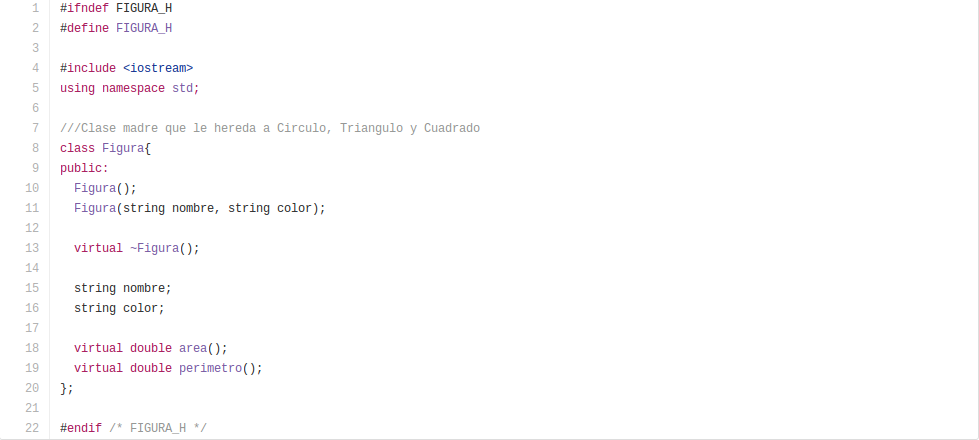
\includegraphics[height=8cm, width=\textwidth]{img/figurah.png}}
\subfigure[Figura.cpp]{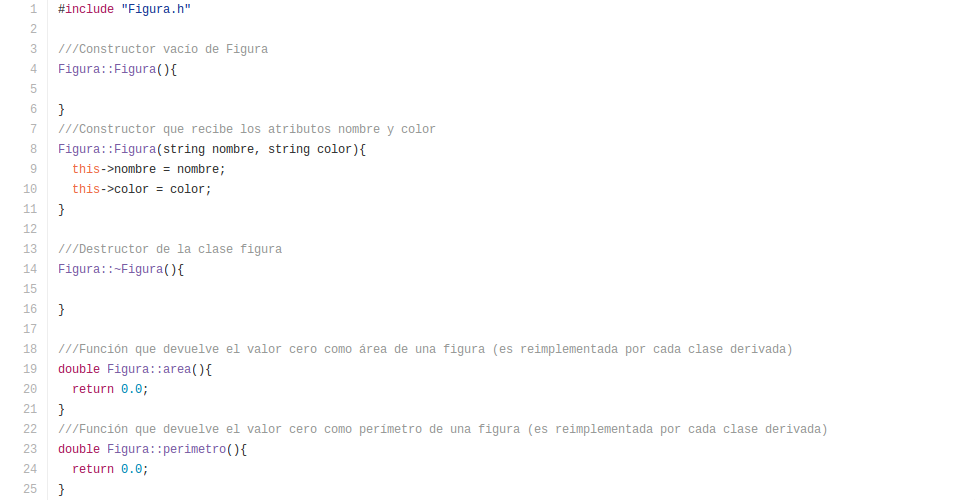
\includegraphics[height=8cm, width=\textwidth]{img/figuracpp.png}}
\caption{Clase base Figura}
\label{fig:base}
\end{figure}

\newpage
\begin{enumerate}

\item Figura.h : se declara el constructor, destructor, los atributos y las funciones que contiene la clase Figura.

  \begin{itemize}
  \item Atributos: dos \textit{string} nombre y color que puede o no recibir el constructor.
  \end{itemize}

\item Figura.cpp : En este archivo se implementan las funciones definidas en Figura.h, por lo que se tiene que incluir en este archivo.
 
 \begin{itemize}
   \item Área: Retorna un double. Se implementa de nuevo en las clases derivadas, por lo que se define como virtual.
   \item Perímetro: Retorna un double. Se implementa de nuevo en las clases derivadas, por lo que se define como virtual.
  \end{itemize}

\end{enumerate}

\newpage
%%%%%%%%%%%%%%%%%%%%%%
\subsection{Clases derivadas}
%%%%%%%%%%%%%%%%%%%%%%

Las clases derivadas son clases en las cuales se utilizó herencia con la clase madre Figura; por lo mismo, se tuvo que incluir el archivo "Figura.h". Sin embargo, cada clase cuenta con ciertos atributos propios de la misma y funciones para acoplar el objetivo a la figura específica. 

Se crearon tres clases derivadas, como se presenta a continuación:

%%%%%%%%%%%%%%%
\subsubsection{Triángulo}
%%%%%%%%%%%%%%%

\begin{figure}[H]
\centering
\subfigure[Triangulo.h]{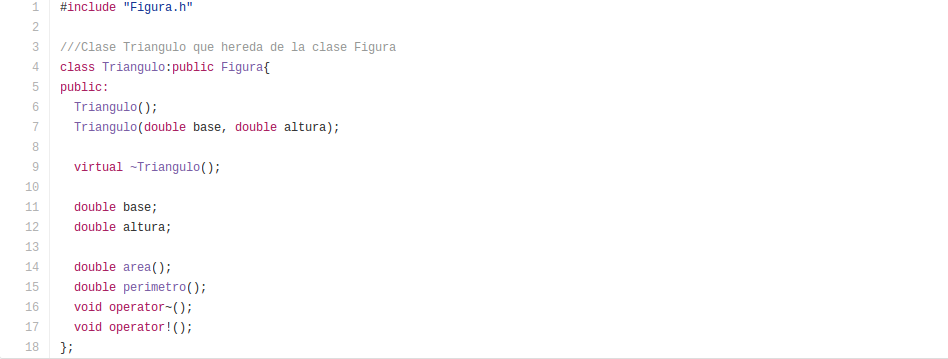
\includegraphics[height=6cm, width=\textwidth]{img/trianguloh.png}}
\subfigure[Triangulo.cpp]{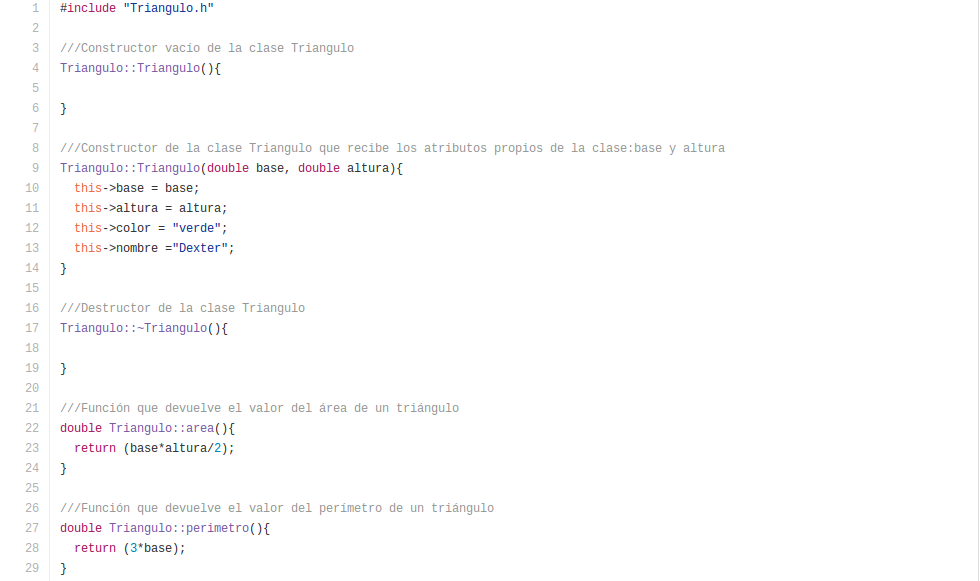
\includegraphics[height=8cm, width=\textwidth]{img/triangulocpp.png}}
\caption{Clase Triangulo derivada de Figura}
\label{fig:tri}
\end{figure}

\newpage
En la línea 4 del archivo Triangulo.h (Figura \ref{fig:tri}) se observa la implementación de la herencia. Además, como se aprecia en la Figura \ref{fig:tri} hay dos atributos adicionales para el Triángulo, el valor de su base y altura.
En el archivo Triangulo.cpp es donde se aprecia la implementación de las funciones de área y perímetro.

\begin{enumerate}
 \item Atributos: dos \textit{double}, base y altura.
 \item Funciones:
	\begin{itemize}
    \item Área: se utiliza la fórmula $A_{triangulo}=\frac{base*altura}{2}$, propia del área del tríangulo.
    \item Perímetro: se utiliza la fórmula $P_{triangulo}=3*base$, propia del perímetro del tríangulo equilátero (Se generalizó la fórmula por comodidad).
    \end{itemize}
\end{enumerate}

%%%%%%%%%%%%%%%%%
\subsubsection{Cuadrado}
%%%%%%%%%%%%%%%%%

\begin{figure}[H]
\centering
\subfigure[Cuadrado.h]{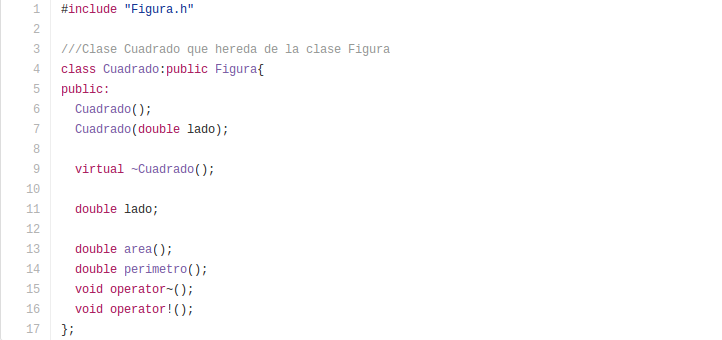
\includegraphics[height=6cm, width=\textwidth]{img/cuadradoh.png}}
\subfigure[Cuadrado.cpp]{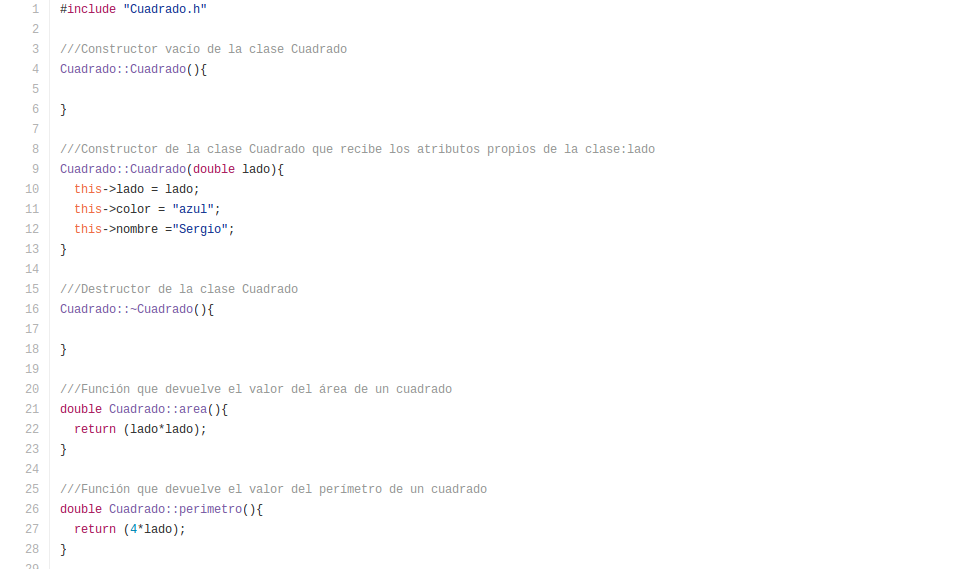
\includegraphics[height=8cm, width=\textwidth]{img/cuadradocpp.png}}
\caption{Clase Cuadrado derivada de Figura}
\label{fig:cua}
\end{figure}

En la línea 4 del archivo Cuadrado.h (Figura \ref{fig:cua}) se observa la implementación de herencia.Se puede apreciar en la Figura que hay un atributo adicional para el Cuadrado, el valor de su lado.En el archivo Cuadrado.cpp es donde se aprecia la implementación de las funciones de área y perímetro.

\begin{enumerate}
 \item Atributos: un \textit{double} lado.
 \item Funciones:
	\begin{itemize}
    \item Área: se utiliza la fórmula $A_{cuadrado}= lado^{2}$, propia del área de un cuadrado.
    \item Perímetro: se utiliza la fórmula $P_{cuadrado}=4*lado$, propia del perímetro de un cuadrado.
    \end{itemize}
\end{enumerate}

%%%%%%%%%%%%%%%%%%
\subsubsection{Círculo}
%%%%%%%%%%%%%%%%%%

\begin{figure}[H]
\centering
\subfigure[Circulo.h]{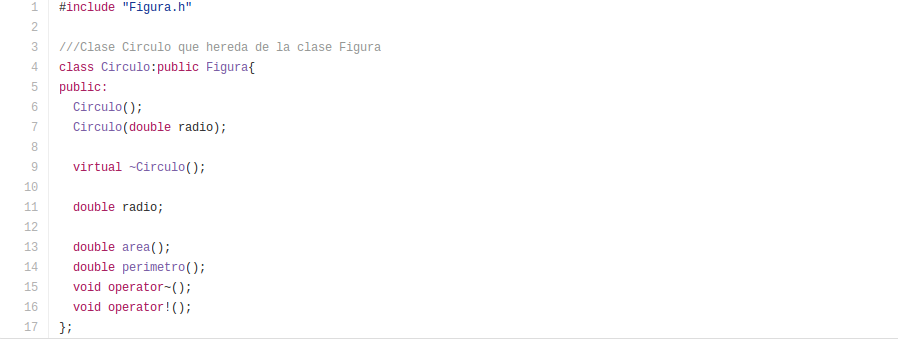
\includegraphics[height=6cm, width=\textwidth]{img/circuloh.png}}
\subfigure[Circulo.cpp]{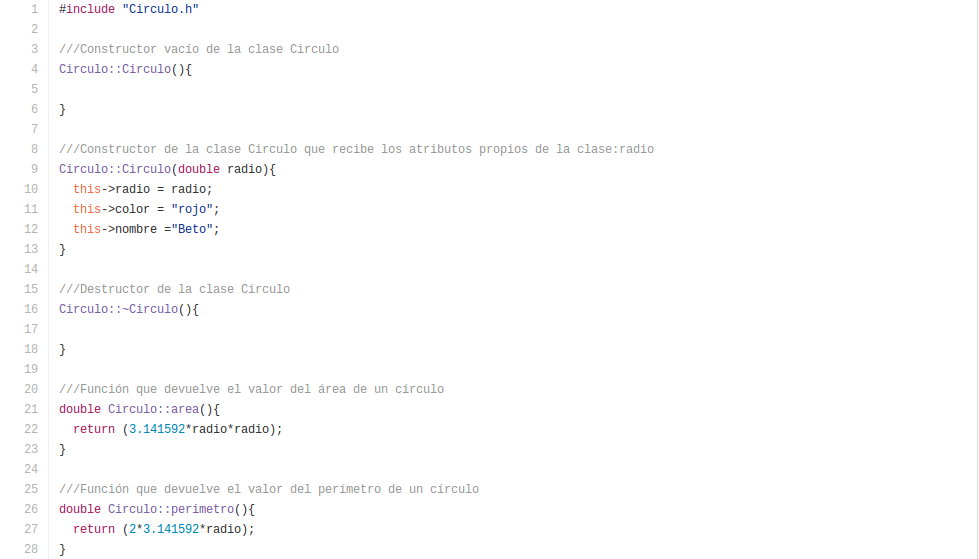
\includegraphics[height=8cm, width=\textwidth]{img/circulocpp.png}}
\caption{Clase Circulo derivada de Figura}
\label{fig:cir}
\end{figure}

En la línea 4 del archivo Circulo.h (Figura \ref{fig:cir}) se observa la implementación de herencia. Se puede apreciar en la Figura  que hay un atributo adicional para el Círculo, el valor de su radio.
En el archivo Circulo.cpp, es donde se aprecia la implementación de las funciones de área y perímetro.

\begin{enumerate}
 \item Atributos: un \textit{double} radio.
 \item Funciones:
	\begin{itemize}
    \item Área: se utiliza la fórmula $A_{circulo}= \pi *r^{2}$, propia del área del círculo.
    \item Perímetro: se utiliza la fórmula $P_{circulo}= 2*\pi *r$, propia del perímetro del círculo.
    \end{itemize}
\end{enumerate}

%%%%%%%%%%%%%%%%%%%%%%
\subsection{Sobrecarga de operadores}
%%%%%%%%%%%%%%%%%%%%%%
La sobrecarga de operadores se utilizó con los operadores ! y $\sim$ para que, al llamar al primero, se imprimieran los datos de cada figura y al llamar al segundo se imprimieran los valores de área y perímetro respectivos. A continuación se presenta la implementación mencionada:

\begin{figure}[H]
\centering
\subfigure[Tríangulo.cpp]{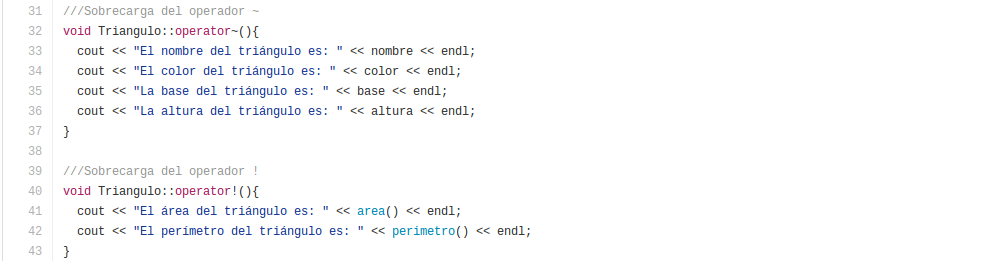
\includegraphics[height=5cm, width=15cm]{img/sobrecargatri.png}}
\subfigure[Circulo.cpp]{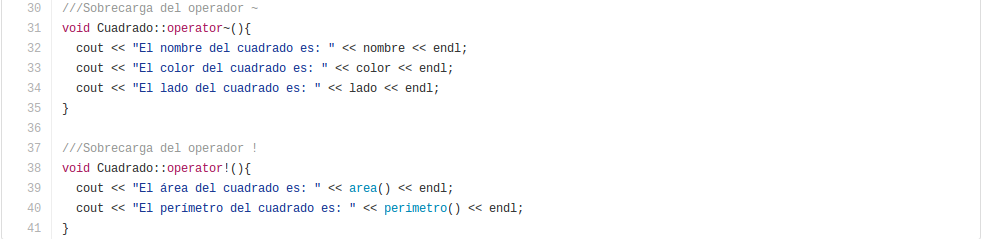
\includegraphics[height=5cm, width=15cm]{img/sobrecargacua.png}}
\subfigure[Circulo.h]{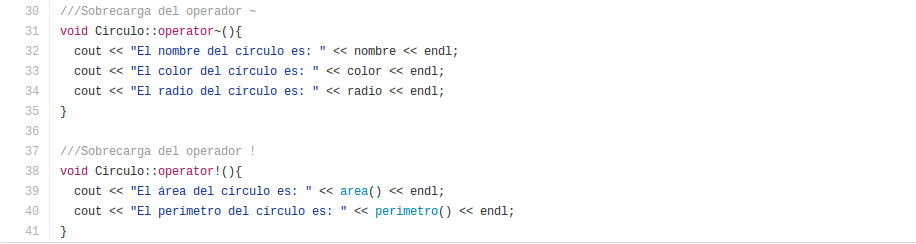
\includegraphics[height=5cm, width=15cm]{img/sobrecargacir.png}}
\caption{Sobrecarga de operadores}
\label{fig:sobrecarga}
\end{figure}

Para realizar la sobrecarga de los operadores, también hay que declarar dichas funciones (tipo void) en los headers, esto se muestro en las figuras \ref{fig:tri}, \ref{fig:cua} y \ref{fig:cir} en las líneas 15-17.

%%%%%%%%%%%%%%%%%%%%%%
\subsection{Main}
%%%%%%%%%%%%%%%%%%%%%%
En el archivo main.cpp se incluyeron todos los archivos headers con el fin de poder hacer uso de los objetos respectivos. 
Se creó un objeto de cada clase derivada, estableciendo sus atributos para luego calcular área y perímetro de éstos. Además, se le aplicaron los operadores sobrecargados a los objetos Triangulo, Circulo y Cuadrado.
 
\begin{figure}[H]
\centering
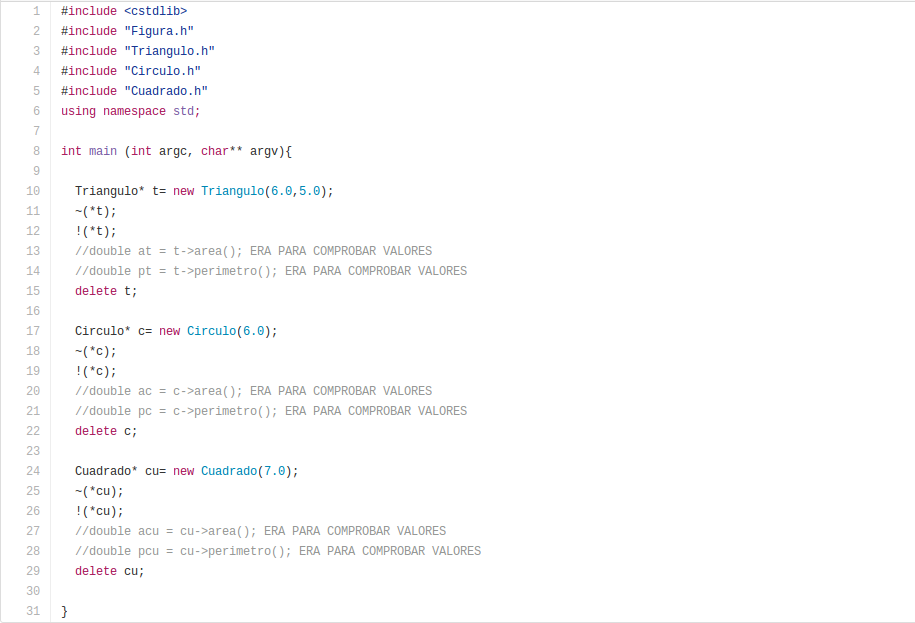
\includegraphics[height=14cm, width=\textwidth]{img/main.png}
\caption{Contenido de main.cpp}
\label{fig:main}
\end{figure}

\newpage
Y su ejecución: 

\begin{figure}[H]
\centering
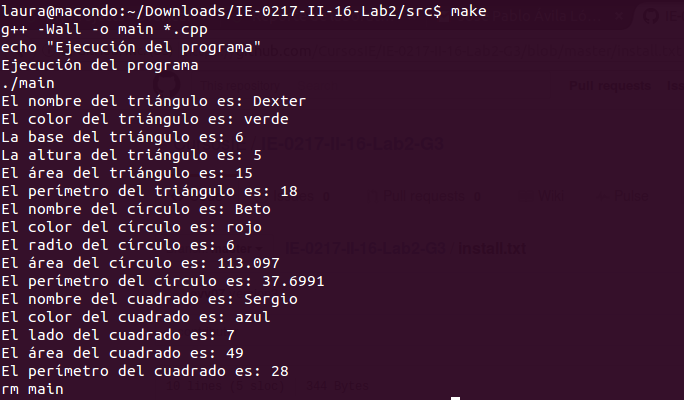
\includegraphics[height=10cm, width=\textwidth]{img/ejecucion.png}
\caption{ejecución del main}
\label{fig:ejecucion}
\end{figure}

\newpage
%%%%%%%%%%%%%%%%%%%%%%
\subsection{Diagrama de clases}
%%%%%%%%%%%%%%%%%%%%%%
Para una mejor visualización de la composición de la clase base y sus derivadas, se presenta a continuación un diagrama de clases:

\begin{figure}[H]
\centering
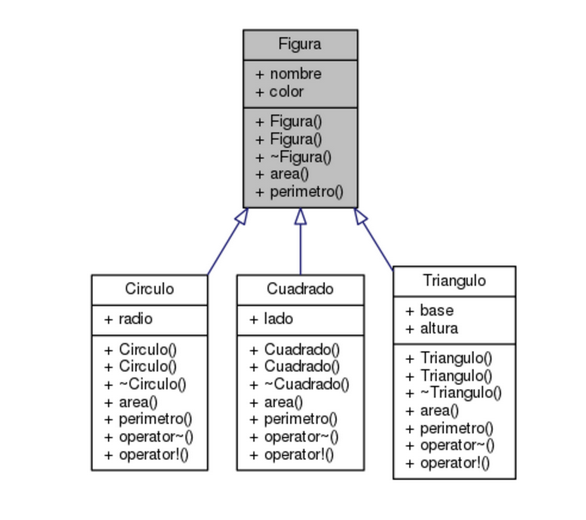
\includegraphics[height=15cm, width=\textwidth]{img/DC.png}
\caption{Diagrama de clases}
\label{fig:diagrama}
\end{figure}


\newpage
%%%%%%%%%%%%%%%%%%%%%%%%%%%%%%%%
\section{Conclusiones}
%%%%%%%%%%%%%%%%%%%%%%%%%%%%%%%%
\begin{itemize}
\item Se empleó la Programación Orientada a Objetos, para el uso de clases.
\item Se logró heredar atributos y características de la clase base a sus clases derivadas.
\item Se implementó el poliformismo para que cada clase reimplementara funciones según sus requerimientos.
\item Se sobrecargaron los operadores ! y $\sim$ para que cumplieran una función determinada al usarse con objetos.
\end{itemize}


\end{document}
